\documentclass[tikz, border=1cm]{standalone}
\usetikzlibrary{fit}

% color shades in HEX
\definecolor{level-2}{HTML}{0082ce}
\definecolor{level-1}{HTML}{009bf5}
\definecolor{level0}{HTML}{31b3ff}
\definecolor{level+1}{HTML}{58c1ff}
\definecolor{level+2}{HTML}{7fd0ff}

\begin{document}

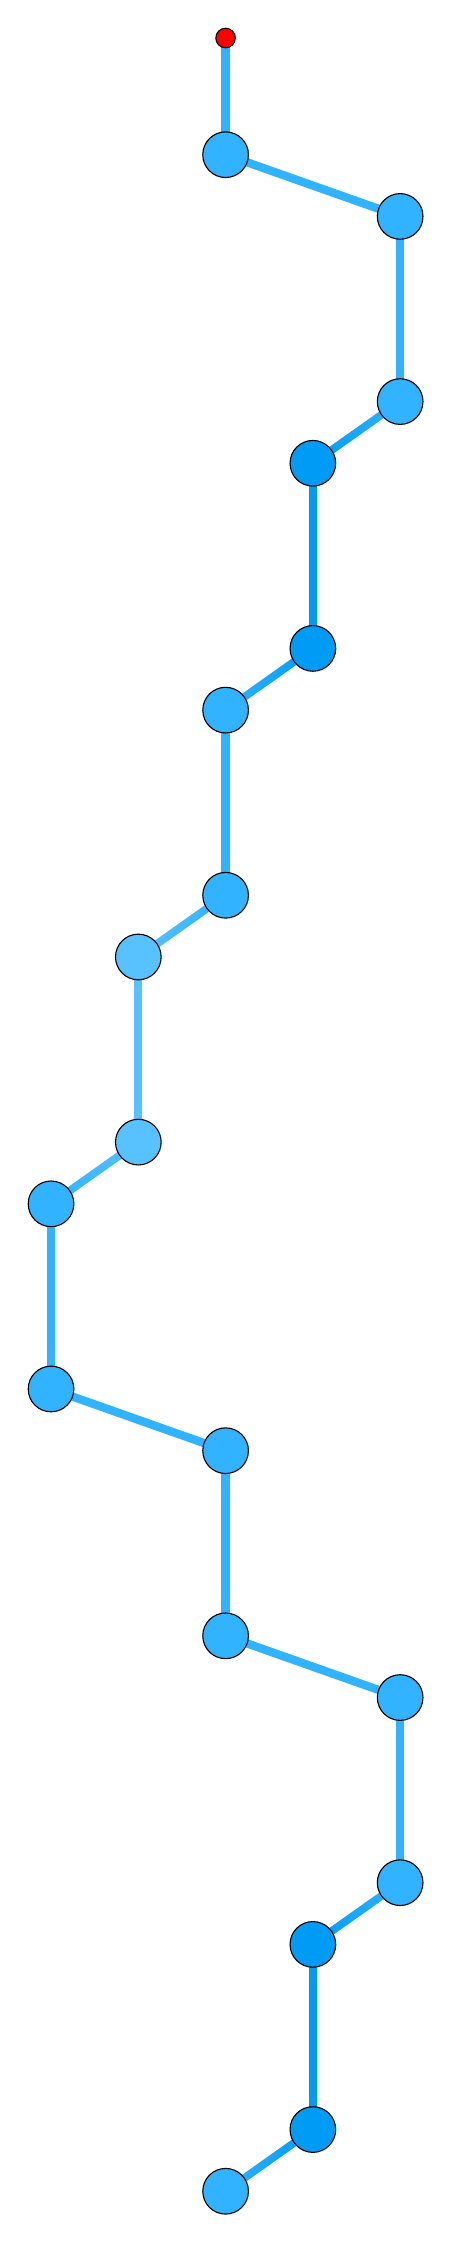
\begin{tikzpicture} % 'xz' side view, with -y coming out of the page

%% coordinates from file
\coordinate (h01)  at ( 0.00000000000000,  28.52186817612748);
\coordinate (si01) at ( 0.00000000000000,  27.03947817579129);
\coordinate (si02) at ( 2.21678821772147,  26.25572518518865);
\coordinate (si03) at ( 2.21678821772147,  23.90446621338074);
\coordinate (si04) at ( 1.10839410886073,  23.12071322277810);
\coordinate (si05) at ( 1.10839410886073,  20.76945425097014);
\coordinate (si06) at ( 0.00000000000000,  19.98570126036750);
\coordinate (si07) at ( 0.00000000000000,  17.63444228855953);
\coordinate (si08) at (-1.10839410886073,  16.85068929795689);
\coordinate (si09) at (-1.10839410886073,  14.49943032614898);
\coordinate (si10) at (-2.21678821772147,  13.71567733554634);
\coordinate (si11) at (-2.21678821772147,  11.36441836373838);
\coordinate (si12) at ( 0.00000000000000,  10.58066537313574);
\coordinate (si13) at ( 0.00000000000000,   8.22940640132778);
\coordinate (si14) at ( 2.21678821772147,   7.44565341072513);
\coordinate (si15) at ( 2.21678821772147,   5.09439443891722);
\coordinate (si16) at ( 1.10839410886073,   4.31064144831458);
\coordinate (si17) at ( 1.10839410886073,   1.95938247650662);
\coordinate (si18) at ( 0.00000000000000,   1.17562948590398);

%% bonds
\draw [line width=3pt, level0]  (h01.center) -- (si01.center);
\draw [line width=3pt, level0]  (si01.center) -- (si02.center);
\draw [line width=3pt, level0]  (si02.center) -- (si03.center);
\path [rotate=35.3, left color=level-1, right color=level0]
        ([shift={(-0.05, 0.05)}] si03) rectangle ([shift={(0.05, -0.05)}] si04);
\draw [line width=3pt, level-1] (si04.center) -- (si05.center);
\path [rotate=35.3, left color=level0, right color=level-1]
        ([shift={(-0.05, 0.05)}] si05) rectangle ([shift={(0.05, -0.05)}] si06);
\draw [line width=3pt, level0]  (si06.center) -- (si07.center);
\path [rotate=35.3, left color=level+1, right color=level0]
        ([shift={(-0.05, 0.05)}] si07) rectangle ([shift={(0.05, -0.05)}] si08);
\draw [line width=3pt, level+1] (si08.center) -- (si09.center);
\path [rotate=35.3, left color=level0, right color=level+1]
        ([shift={(-0.05, 0.05)}] si09) rectangle ([shift={(0.05, -0.05)}] si10);
\draw [line width=3pt, level0]  (si10.center) -- (si11.center);
\draw [line width=3pt, level0]  (si11.center) -- (si12.center);
\draw [line width=3pt, level0]  (si12.center) -- (si13.center);
\draw [line width=3pt, level0]  (si13.center) -- (si14.center);
\draw [line width=3pt, level0]  (si14.center) -- (si15.center);
\path [rotate=35.3, left color=level-1, right color=level0]
        ([shift={(-0.05, 0.05)}] si15) rectangle ([shift={(0.05, -0.05)}] si16);
\draw [line width=3pt, level-1] (si16.center) -- (si17.center);
\path [rotate=35.3, left color=level0, right color=level-1]
        ([shift={(-0.05, 0.05)}] si17) rectangle ([shift={(0.05, -0.05)}] si18);

%% atoms
\node [scale=0.75, circle, draw=black, fill=red] at (h01) {};
\node [scale=1.75, circle, draw=black, fill=level0 ] at (si01) {};
\node [scale=1.75, circle, draw=black, fill=level0 ] at (si02) {};
\node [scale=1.75, circle, draw=black, fill=level0 ] at (si03) {};
\node [scale=1.75, circle, draw=black, fill=level-1] at (si04) {};
\node [scale=1.75, circle, draw=black, fill=level-1] at (si05) {};
\node [scale=1.75, circle, draw=black, fill=level0 ] at (si06) {};
\node [scale=1.75, circle, draw=black, fill=level0 ] at (si07) {};
\node [scale=1.75, circle, draw=black, fill=level+1] at (si08) {};
\node [scale=1.75, circle, draw=black, fill=level+1] at (si09) {};
\node [scale=1.75, circle, draw=black, fill=level0 ] at (si10) {};
\node [scale=1.75, circle, draw=black, fill=level0 ] at (si11) {};
\node [scale=1.75, circle, draw=black, fill=level0 ] at (si12) {};
\node [scale=1.75, circle, draw=black, fill=level0 ] at (si13) {};
\node [scale=1.75, circle, draw=black, fill=level0 ] at (si14) {};
\node [scale=1.75, circle, draw=black, fill=level0 ] at (si15) {};
\node [scale=1.75, circle, draw=black, fill=level-1] at (si16) {};
\node [scale=1.75, circle, draw=black, fill=level-1] at (si17) {};
\node [scale=1.75, circle, draw=black, fill=level0 ] at (si18) {};
\end{tikzpicture}



\end{document}
